\pagestyle{acorde}
\label{acorde}
%\begin{textblock*}{5.625in}(0pt,0pt)%
%\vspace*{-3.5cm}
%\hspace*{-2.77cm}\includegraphics*[width=175.2mm]{./propagandas/IMA.pdf}
%\end{textblock*}
%\pagebreak

\begin{center}
\hspace*{.5cm}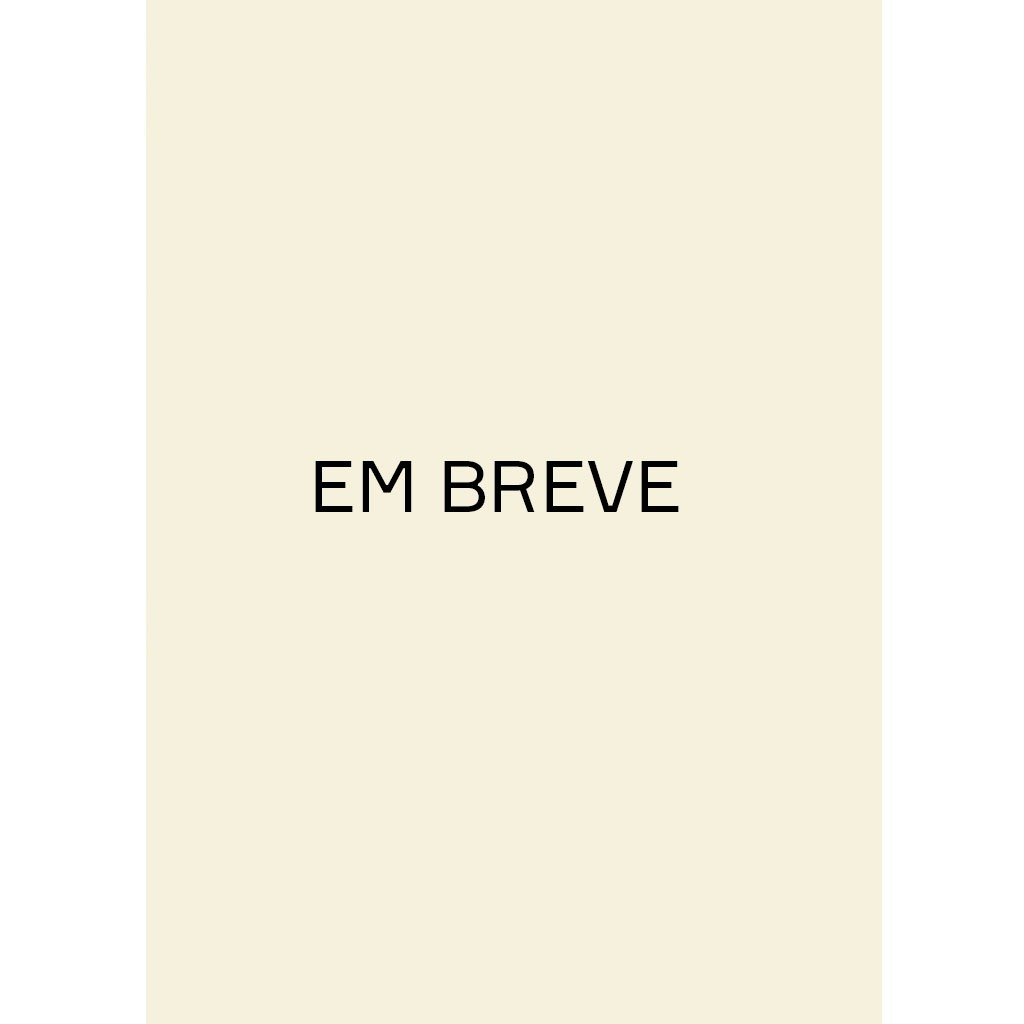
\includegraphics[width=74mm]{./CAPAS/breve.jpeg}
\end{center}
\hspace*{-7cm}\hrulefill\hspace*{-7cm}
\medskip

\noindent{}Inserir.

\vfill
\hspace*{-.4cm}\begin{minipage}[c]{.5\linewidth}
\small\textbf{
\hspace*{-.1cm}Editora: Acorde\\
Título: Luiz Tatit: no princípio era o meio\\
Autor: Luís Augusto Fischer\\ 
ISBN: 978-65-994412-9-5\\
Páginas: Inserir.\\
Formato: Inserir.\\
Preço: R\$ Inserir.\\
}
\end{minipage}
\pagebreak

\begin{center}
\hspace*{.5cm}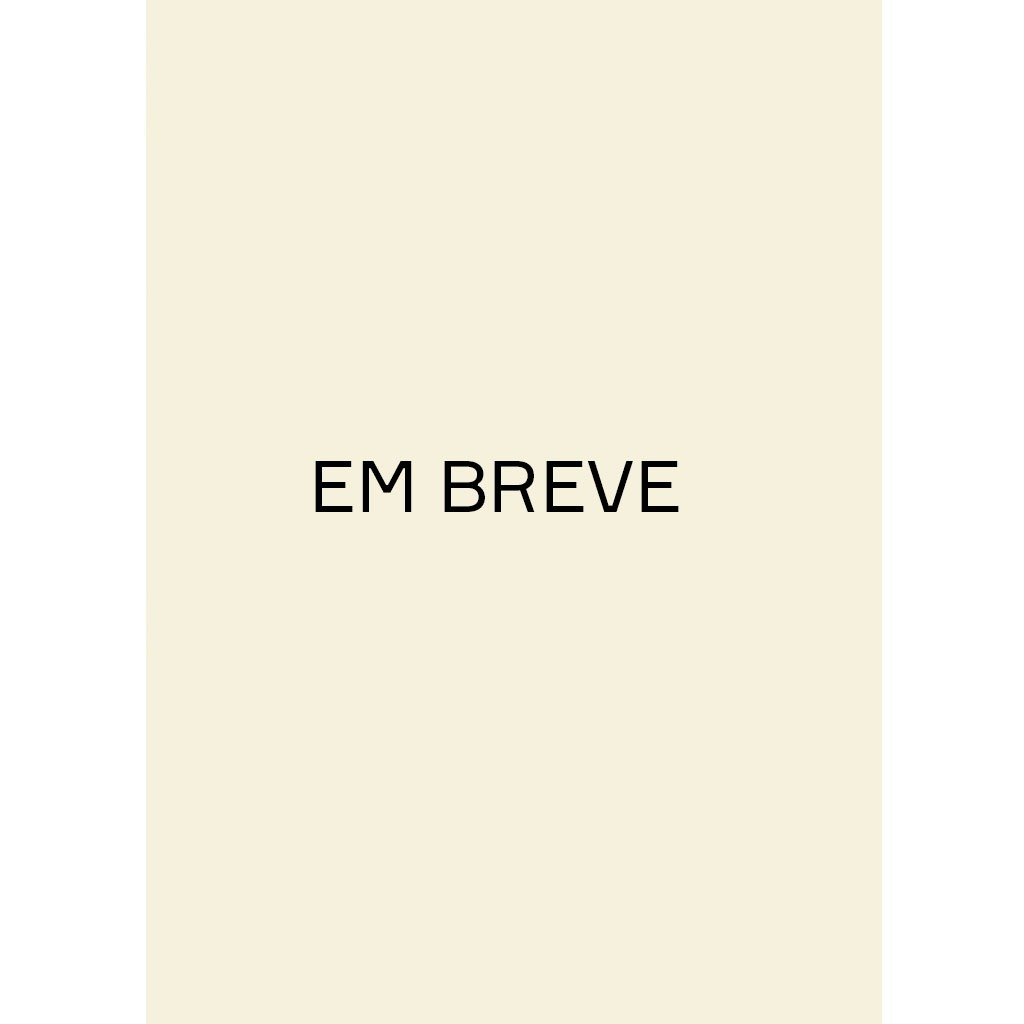
\includegraphics[width=74mm]{./CAPAS/breve.jpeg}
\end{center}
\hspace*{-7cm}\hrulefill\hspace*{-7cm}
\medskip

\noindent{}Inserir.

\vfill
\hspace*{-.4cm}\begin{minipage}[c]{.5\linewidth}
\small\textbf{
\hspace*{-.1cm}Editora: Acorde\\
Título: Mário de Andrade: a estranha\\força da canção\\
Autor: Marcos Lacerda\\ 
ISBN: 978-65-994412-8-8\\
Páginas: Inserir.\\
Formato: Inserir.\\
Preço: R\$ Inserir.\\
}
\end{minipage}
\pagebreak

\vspace*{1.5cm}
\noindent{}{\nohyphens{\LARGE{Texto}}}
\bigskip

\hfill{}\scalebox{.8}{AUTOR}
\bigskip
\bigskip
\bigskip

\begin{multicols}{2}
\noindent{}Mussum Ipsum, cacilds vidis litro abertis. Atirei o pau no gatis, per gatis num morreus. Leite de capivaris, leite de mula manquis sem cabeça. Praesent malesuada urna nisi, quis volutpat erat hendrerit non. Nam vulputate dapibus. Suco de cevadiss, é um leite divinis, qui tem lupuliz, matis, aguis e fermentis.

Tá deprimidis, eu conheço uma cachacis que pode alegrar sua vidis. Suco de cevadiss deixa as pessoas mais interessantis. In elementis mé pra quem é amistosis quis leo. Quem num gosta di mim que vai caçá sua turmis!

Viva Forevis aptent taciti sociosqu ad litora torquent. Mauris nec dolor in eros commodo tempor. Aenean aliquam molestie leo, vitae iaculis nisl. Posuere libero varius. Nullam a nisl ut ante blandit hendrerit. Aenean sit amet nisi. Vehicula non. Ut sed ex eros. Vivamus sit amet nibh non tellus tristique interdum.

Em pé sem cair, deitado sem dormir, sentado sem cochilar e fazendo pose. Detraxit consequat et quo num tendi nada. Pra lá , depois divoltis porris, paradis. Per aumento de cachacis, eu reclamis.

Quem manda na minha terra sou euzis! A ordem dos tratores não altera o pão duris. Paisis, filhis, espiritis santis. Aenean aliquam molestie leo, vitae iaculis nisl.

Diuretics paradis num copo é motivis de denguis. Mais vale um bebadis conhecidiss, que um alcoolatra anonimis. Sapien in monti palavris qui num significa nadis i pareci latim. Admodum accumsan disputationi eu sit. Vide electram sadipscing et per.

Manduma pindureta quium dia nois paga. Interagi no mé, cursus quis, vehicula ac nisi. Praesent vel viverra nisi. Mauris aliquet nunc non turpis scelerisque, eget. Casamentiss faiz malandris se pirulitá.

Quem num gosta di mé, boa gentis num é. Si num tem leite então bota uma pinga aí cumpadi! Todo mundo vê os porris que eu tomo, mas ninguém vê os tombis que eu levo! Cevadis im ampola pa arma uma pindureta.

\vspace{\baselineskip}
{\small\fakereceipt{
\noindent{}Diuretics paradis num copo é motivis de denguis. Mais vale um bebadis conhecidiss, que um alcoolatra anonimis. Sapien in monti palavris qui num significa nadis i pareci latim. Admodum accumsan disputationi eu sit. Vide electram sadipscing et per.
}}
\vspace{\baselineskip}

Mussum Ipsum, cacilds vidis litro abertis. Atirei o pau no gatis, per gatis num morreus. Leite de capivaris, leite de mula manquis sem cabeça. Praesent malesuada urna nisi, quis volutpat erat hendrerit non. Nam vulputate dapibus. Suco de cevadiss, é um leite divinis, qui tem lupuliz, matis, aguis e fermentis.

Tá deprimidis, eu conheço uma cachacis que pode alegrar sua vidis. Suco de cevadiss deixa as pessoas mais interessantis. In elementis mé pra quem é amistosis quis leo. Quem num gosta di mim que vai caçá sua turmis!

Viva Forevis aptent taciti sociosqu ad litora torquent. Mauris nec dolor in eros commodo tempor. Aenean aliquam molestie leo, vitae iaculis nisl. Posuere libero varius. Nullam a nisl ut ante blandit hendrerit. Aenean sit amet nisi. Vehicula non. Ut sed ex eros. Vivamus sit amet nibh non tellus tristique interdum.

Em pé sem cair, deitado sem dormir, sentado sem cochilar e fazendo pose. Detraxit consequat et quo num tendi nada. Pra lá , depois divoltis porris, paradis. Per aumento de cachacis, eu reclamis.

Quem manda na minha terra sou euzis! A ordem dos tratores não altera o pão duris. Paisis, filhis, espiritis santis. Aenean aliquam molestie leo, vitae iaculis nisl.

Diuretics paradis num copo é motivis de denguis. Mais vale um bebadis conhecidiss, que um alcoolatra anonimis. Sapien in monti palavris qui num significa nadis i pareci latim. Admodum accumsan disputationi eu sit. Vide electram sadipscing et per.

Manduma pindureta quium dia nois paga. Interagi no mé, cursus quis, vehicula ac nisi. Praesent vel viverra nisi. Mauris aliquet nunc non turpis scelerisque, eget. Casamentiss faiz malandris se pirulitá.

Quem num gosta di mé, boa gentis num é. Si num tem leite então bota uma pinga aí cumpadi! Todo mundo vê os porris que eu tomo, mas ninguém vê os tombis que eu levo! Cevadis im ampola pa arma uma pindureta.

\bigskip
\noindent{}\textcolor{gray}{\footnotesize\slsc{\textls[-15]{Texto tal tal e tal.}}}
\end{multicols}

\pagebreak
\pagestyle{acordecat}
\begin{multicols}{2}
\begin{enumerate}
\raggedright\nohyphens{
\item Marcelino, \textbf{Godofredo De Oliveira Neto}
\item Desamores da portuguesa, \textbf{Marta Barbosa Stephens}
\item Clube da esquina - Milton Nascimento e Lô Borges, \textbf{Milton Nascimento; Lô Borges; Charles Gavin}
\item Parasito, \textbf{Andrea Rangel}
\item Academia de danças - Egberto Gismonti, \textbf{Egberto Gismonti; Charles Gavin}
\item Secos \& Molhados, \textbf{Ney Matogrosso; Gerson Conrad; Charles Gavin}
\item 100 dias em Paris, \textbf{Tania Carvalho}
\item Perdidas, \textbf{Andrea del Fuego; Edney Silvestre; Henrique Rodrigues; Marcelo Moutinho; Marta Barbosa Stephens; Martha Batalha; Kátia Bandeira de Mello  Gerlach; Alexandre Staut} 
\item Rosa de ouro - Aracy Côrtes e Clementina de Jesus, \textbf{Hemínio Bello de Carvalho; Paulinho da Viola; Elton Medeiros; Charles Gavin}
\item Chico Buarque para todos, \textbf{Regina Zappa}
\item Galos de briga - João Bosco, \textbf{João Bosco; Charles Gavin}
\item Quem é quem - João Donato, \textbf{João Donato; Marcos Valle; Charles Gavin}
\item Dois - Legião Urbana, \textbf{Dado Villa-Lobos; Marcelo Bonfá; Charles Gavin}
\item Mulheres que mordem, \textbf{Beatriz Leal}
\item Nervos de aço - Paulinho da Viola, \textbf{Paulinho da Viola; Charles Gavin; Monarco}
\item Sociedade dividida, \textbf{Raphael Lima}
\item Estudando o samba - Tom Zé, \textbf{Tom Zé; Charles Gavin}
\item Reprograme, \textbf{Cory Doctorow; Nina Simon; Jane Finnis; Luis Marcelo Mendes}
\item Como o Botafogo conquistou a China, \textbf{Bruno Porto}
\item A peleja do diabo com o dono do céu -- Zé Ramalho, \textbf{Zé Ramalho; Charles Gavin}
\item A árvore oca, \textbf{Mauricio Vieira}
\item A morte visita Lisboa, \textbf{Fernando Perdigão}
\item Biografia do Língua, \textbf{Mario Lucio Sousa}
\item 100 dias em Lisboa, \textbf{Tania Carvalho}
\item A vagabunda, \textbf{Sidonie Gabrielle Colette}
}
\end{enumerate}
\end{multicols}

\pagebreak